\documentclass[tikz,border=6pt]{standalone}
\usepackage[utf8]{inputenc}
\usepackage[T1]{fontenc}
\usepackage{tikz}
\usetikzlibrary{positioning}
\begin{document}
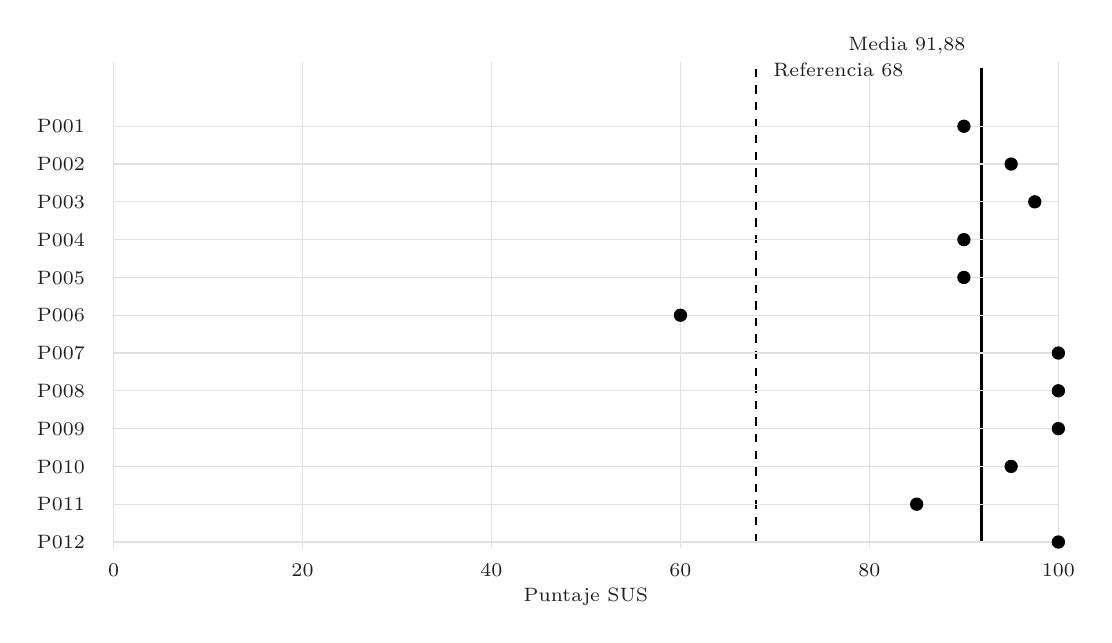
\begin{tikzpicture}[x=0.12cm,y=0.48cm,font=\sffamily]
  \definecolor{ink}{RGB}{32,32,32}
  \definecolor{soft}{RGB}{225,225,225}
  \definecolor{accent}{RGB}{0,0,0}

  \draw[soft, line width=0.4pt] (0,0) -- (100,0);
  \foreach \x in {0,20,40,60,80,100} {
    \draw[soft, line width=0.4pt] (\x,-0.15) -- (\x,12.7);
    \node[ink, font=\scriptsize] at (\x,-0.75) {\x};
  }
  \node[ink, font=\scriptsize] at (50,-1.45) {Puntaje SUS};

  \draw[accent, dashed, line width=0.65pt] (68,0) -- (68,12.55);
  \node[anchor=south west, ink, font=\scriptsize] at (68.8,12.05) {Referencia 68};

  \draw[accent, line width=0.9pt] (91.88,0) -- (91.88,12.55);
  \node[anchor=south east, ink, font=\scriptsize] at (91.2,12.65) {Media 91,88};

  \foreach \code/\score/\row in {
    P001/90/11,
    P002/95/10,
    P003/97.5/9,
    P004/90/8,
    P005/90/7,
    P006/60/6,
    P007/100/5,
    P008/100/4,
    P009/100/3,
    P010/95/2,
    P011/85/1,
    P012/100/0
  } {
    \node[anchor=east, ink, font=\scriptsize] at (-2,\row) {\code};
    \draw[soft, line width=0.4pt] (0,\row) -- (100,\row);
    \filldraw[fill=accent, draw=accent] (\score,\row) circle (2.2pt);
  }
\end{tikzpicture}
\end{document}
